\section{Overview}\label{sec:overview}


%Given a 2D expanded layout of a carton, our system allows users to explore the shape and structure of corresponding models.


 
Figure~\ref{fig:overview} shows the overview of our construction algorithm. 
As shown in Figure~\ref{fig:overview}(a), the input 2D design layout of a carton consists of a set of cutting edges (solid lines) and folding edges (dashed lines).
%
Given the 2D layout, its topology is recovered by finding the minimum edge loops as faces, as Figure~\ref{fig:overview}(b) shows. Each face is filled with a unique color. %by ignoring the holes in the plane
The 2D layout therefore can be represented by a polymesh $L=(V,E,F)$, where $V$ is the set of vertexes, $E$ is the set of all edges, and $F$ is the set of faces. 
The edge set $E=E_c\cup E_f$, where $E_c$ is the set of cutting edges, and $E_f$ is the set of folding edges.
%
To build a 3D model $M={V, E, F}$ from the 2D layout $L$, while they share the same topology, we compute the 3D coordinates of all vertexes in $V$. 
%
Our algorithm consists of two steps. 
First, an initial 3D model (Figure~\ref{fig:overview}(c)) is constructed by given a specific angle to each folding edge, which will be explained later in Sec.~\ref{sec:initialization}.
The user can then manipulate and explore 3D shapes of the canton based on a series of suggestive operation provided by our system. 
%
The final model is shown in Figure~\ref{fig:overview}(d).
% is finally built through the optimization based on the information acquired from user interaction. 

\comments{
  a flat polymesh $L$ is created from a 2D design layout of a box, then we deform the input polymesh into its 3D realization $R_i$ according to the predicted angles along each of its fold edges, and through optimization, generate final model $R_f$. A polymesh consists of a set of vertices, edges and faces $M = (V,E,F)$, the number of vertexes $V$, edges $E$ and faces $F $ vary from one mesh to another. However, a pair of $(L,R_f)$ as the 2D layout and its corresponding 3D realization share the same topology and therefore they have the same number of vertices, edges and faces. A flat mesh as a 2D layout $L$ has its $z$ component of each vertex set to be a constant zero: $X_z(\mathbf{v}) \equiv 0$ where $X = (X_x,X_y,X_z)$ is the vertex coordinate, and its normal of each face set as $(0,0,1)^T$: $\mathbf{n}(f) \equiv (0,0,1)^T$, where $f \in F$.
}


\begin{figure}
	\centering
	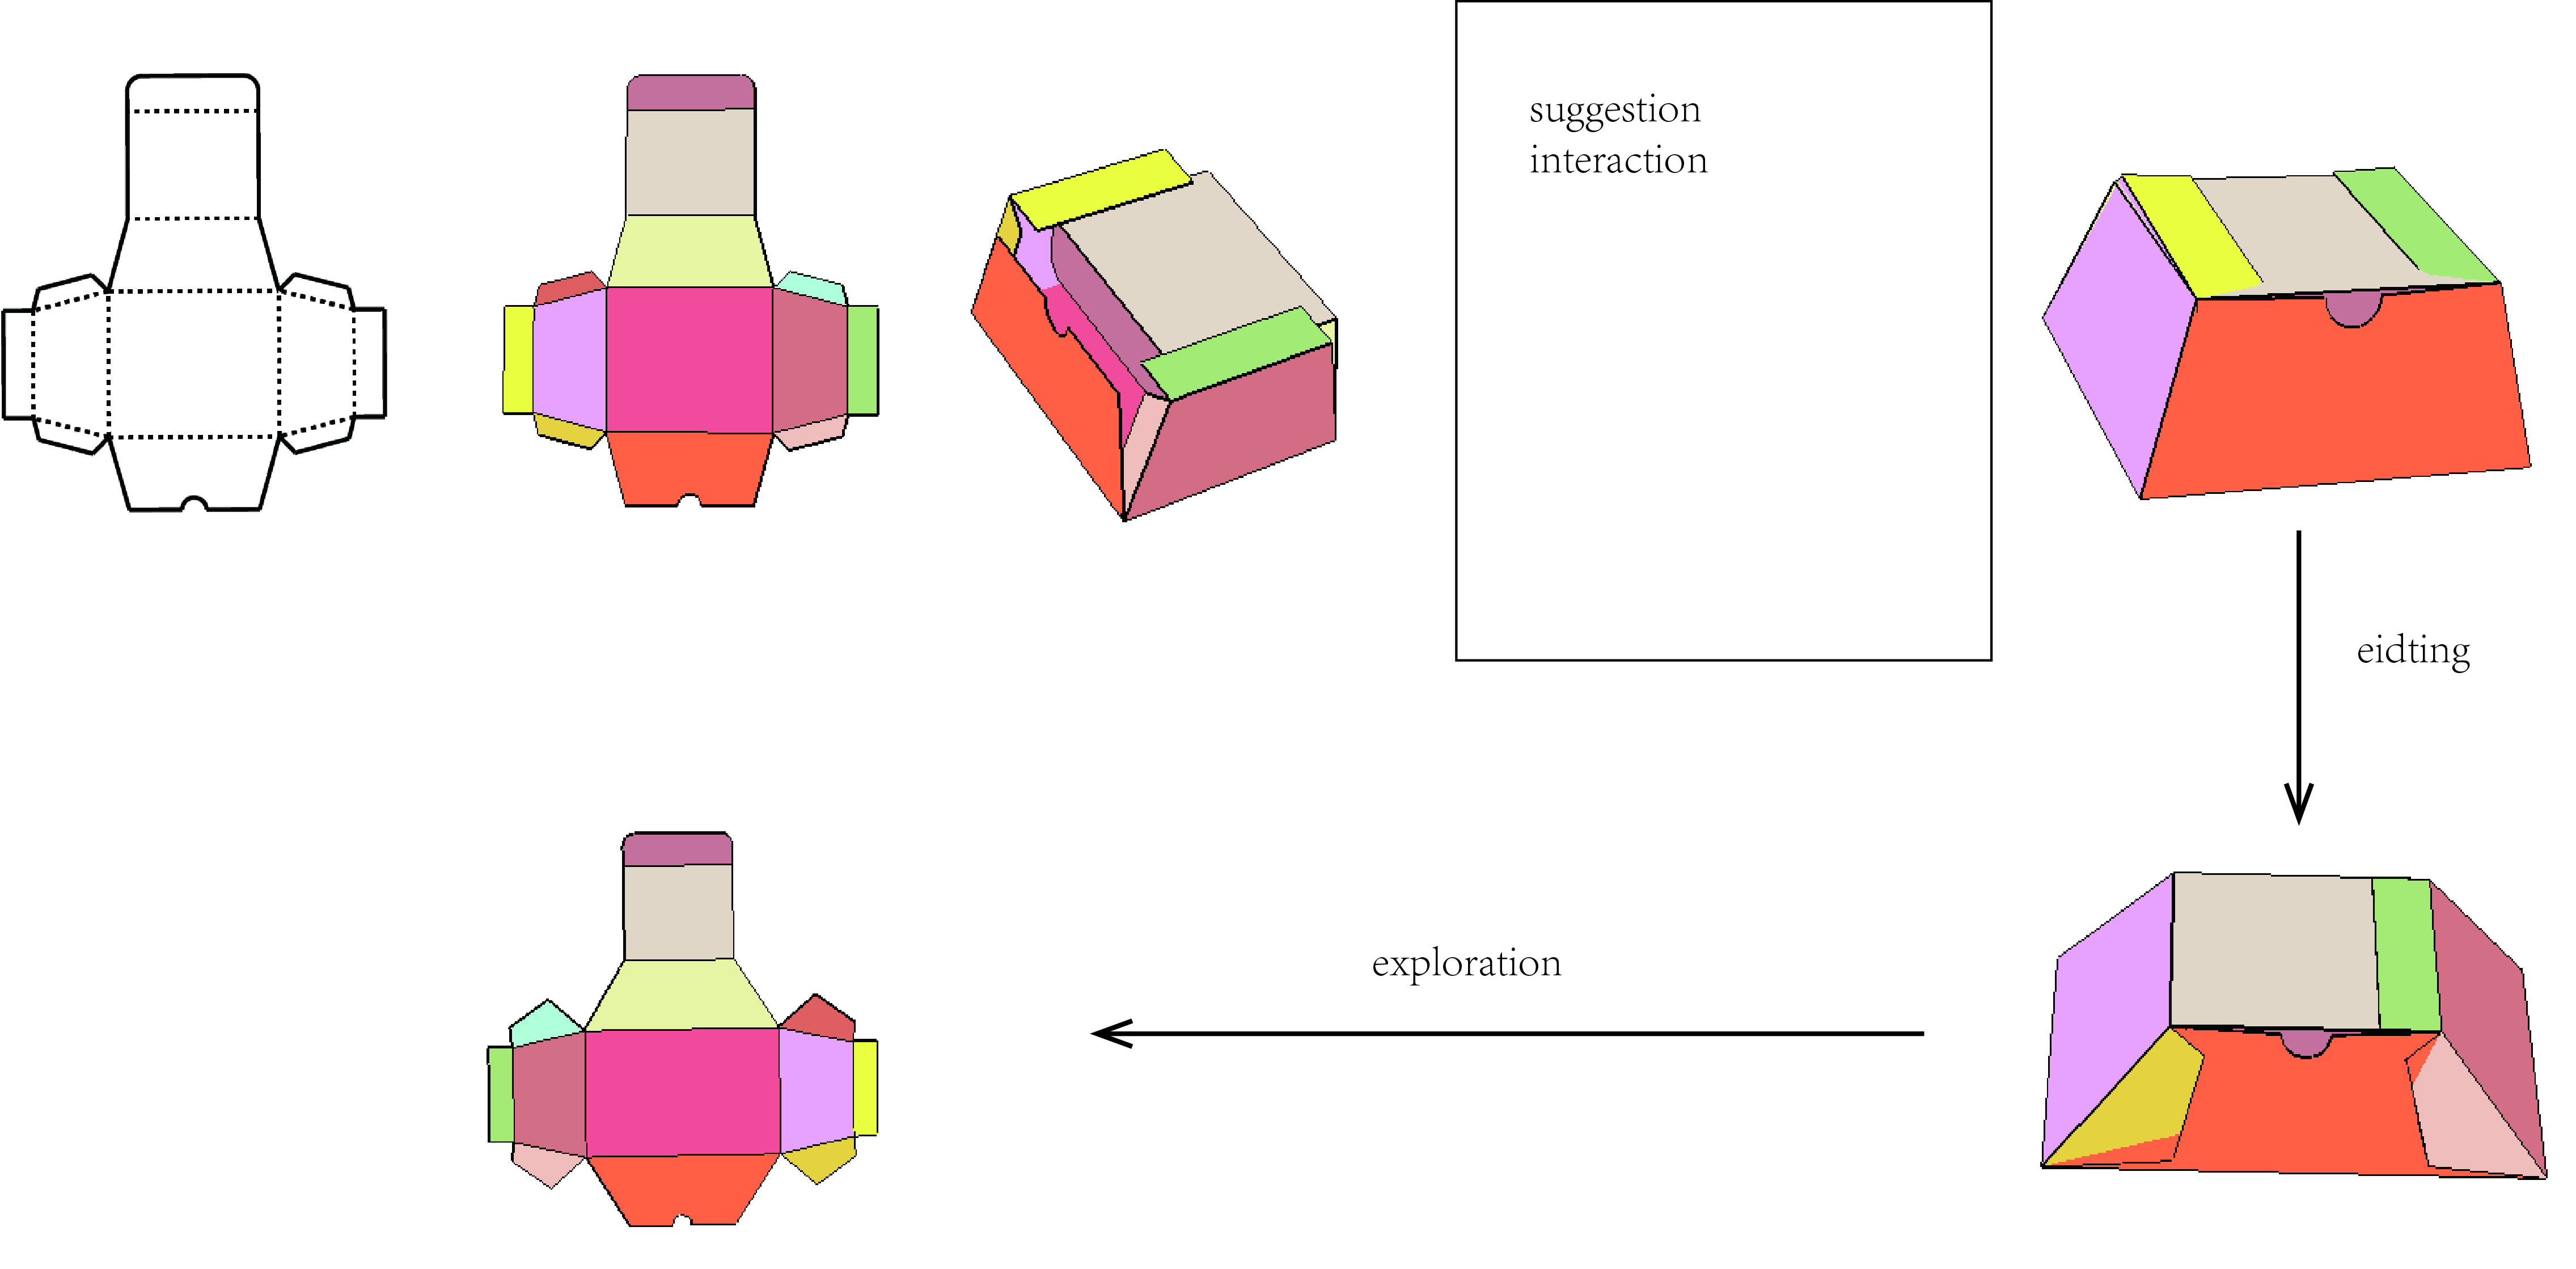
\includegraphics[width=0.9\textwidth]{images/overview.jpg}
	\caption{Given a 2D layout (a), we first extract its 2D mesh (b), with different face in different color. By providing each folding edge with a specific angle, we can construct an initial 3D model (c). The final carton model (d) is built through the shape optimization based on the information acquired from user interactions.}
	\label{fig:overview}
\end{figure} 

